\chapter{Results}
\label{chap:partI_results}

After the training, the four competing architectures and the non-ML baseline were compared in three different scenarios: full design, weight maps only (no AO) and artifacts oversampling only (no WM). 
The 70 full-size images of the test set were used as a testbed.
\Cref{tab:metrics} reports individual model performances in terms of both detection and counting ability.
\begin{table}[H]
\centering
\resizebox{\textwidth}{!}{\begin{tabular}{lrrrrrrrr}
\toprule
Model &  Threshold &      $F_1$ &  Accuracy &  Precision &  Recall &     MAE &  MedAE &     MPE (\%) \\
\midrule
\textbf{c-ResUnet}          &      \textbf{0.875} &  \underline{\textbf{0.8149}} &    \textbf{0.6877} &     0.9081 &  \textbf{0.7391} &  \underline{\textbf{3.0857}} &    \textbf{1.0} & -5.13 \\
c-ResUnet (no AO)  &      0.875 &  0.8047 &    0.6732 &     0.9019 &  0.7264 &  3.0857 &    1.5 & -6.24 \\
c-ResUnet (no WM)  &      0.875 &  0.7613 &    0.6147 &     0.9418 &  0.6389 &  3.6857 &    \textbf{1.0} & -19.14 \\
\midrule
ResUnet            &      0.850 &  0.7855 &    0.6468 &     0.8865 &  0.7052 &  3.3286 &    \textbf{1.0} & \textbf{-4.84} \\
ResUnet (no WM)    &      0.850 &  0.7513 &    0.6016 &     0.9387 &  0.6262 &  4.0571 &    2.0 & -24.12 \\
Unet               &      0.875 &  0.7724 &    0.6291 &     0.9117 &  0.6700 &  3.5143 &    1.5 & -14.36 \\
Unet (no WM)       &      0.850 &  0.7886 &    0.6510 &     0.8989 &  0.7024 &  3.1571 &    2.0 & -9.23 \\
small Unet         &      0.875 &  0.7563 &    0.6081 &     0.9264 &  0.6389 &  3.5714 &    2.0 & -21.37 \\
small Unet (no WM) &      0.825 &  0.6697 &    0.5034 &     \textbf{0.9483} &  0.5176 &  4.7714 &    2.0 & -32.01 \\
\midrule
Adaptive Threshold &      0.994 & 0.6106 &	0.4394 &	0.5680 &	0.6601  &	8.0143 &	6.0000 &	78.2553 \\
\bottomrule
\end{tabular}}
\caption{
Performance metrics computed on the test set using the optimal \textit{kneed} threshold. The first four columns report the detection metrics, while the latter ones evaluate counting performance.
}
\label{tab:metrics}
% \end{center}
\end{table}

% \noindent\textbf{Performance}.
\section{Performance}

By looking at the main figures of merit ($F_1$ score and MAE), it is clear how deep learning approaches perform better than the adaptive thresholding.

c-ResUnet clearly outperforms all competitors.
Remarkably, the Unet is consistently worse than c-ResUnet and ResUnet despite having far more parameters (nearly 14M against 1.7M and 887k, respectively).
The advantage of the ResUnet architectures is even more evident when comparing with the lighter Unet version which has a comparable number of parameters (876k).

In addition, c-ResUnet keeps its leading role also when extending the evaluation to the other metrics.
The only meaningful exception is precision, for which the Unet architectures are better. This is probably due to a tendency to overdetection. 
Nonetheless, the ResUnet counterparts well balance this behaviour with a significant improvement in accuracy and recall.

Finally, it is worth noticing that adopting the kneed optimal threshold ensures large cutoffs and enforces only detections with high confidence.
Although desired, this behavior also increases false negatives as less cells are detected. 
As a result, we observe a drop in the accuracy whereby the impact of false negatives is twice as much the one in the $F_1$ score (cf. \cref{eq:accuracy,eq:F1}), thus explaining the gap between these two metrics.
% As a result, we observe a drop in the measures that are more impacted by false negatives, which explains the lower value of the accuracy compared to the $F_1$ score.
In conclusion, the model provides reliable predictions and satisfies the design requirement of being conservative with counts, as suggested by the negative values of MPE for all experimental conditions.

% \noindent\textbf{Ablation studies}.
\section{Ablation studies}

In order to evaluate the impact of artifacts oversampling and weight maps, the experiments were repeated under the same conditions%
% described in \nameref{sec:model_training}
, alternately switching off one of the two design choices.

From \cref{tab:metrics} it is evident how penalizing errors in crowded areas has a positive impact. Indeed, experiments exploiting weight maps achieve consistently better results than those without this addition (no WM), except for the Unet architecture.  
In particular, this strategy seems to produce a loss in precision to foster a more significant gain in accuracy and recall.
\Cref{fig:weigths_effect} illustrates a visual comparison of c-ResUnet output in crowded areas with (top) and without (bottom) weight maps. 
Again, its beneficial contribution is apparent, with close-by cells sharply separated when exploiting the weight maps.

Regarding the impact of artifacts augmentation, \cref{tab:metrics} shows how there is little difference between the full c-ResUnet and the one without oversampling of challenging examples (no AO).
In particular, the advantage of artifacts oversampling is numerically minimal.
This is also confirmed by qualitative evaluation (\cref{fig:predictions}).
On the one hand, the c-ResUnet (no AO) is able to avoid detecting more evident artifacts as the strip (\cref{fig:predictions:noAO}) even without specific oversampling.
On the other, the c-ResUnet  still fails to ignore more troublesome bright structures (\cref{fig:predictions:artifact}) although additional challenging examples were provided during training.
For this reason, the experiment was not replicated for the other architectures. 
\begin{figure}
% \begin{wrapfigure}{R}{0.55\textwidth}
\centering
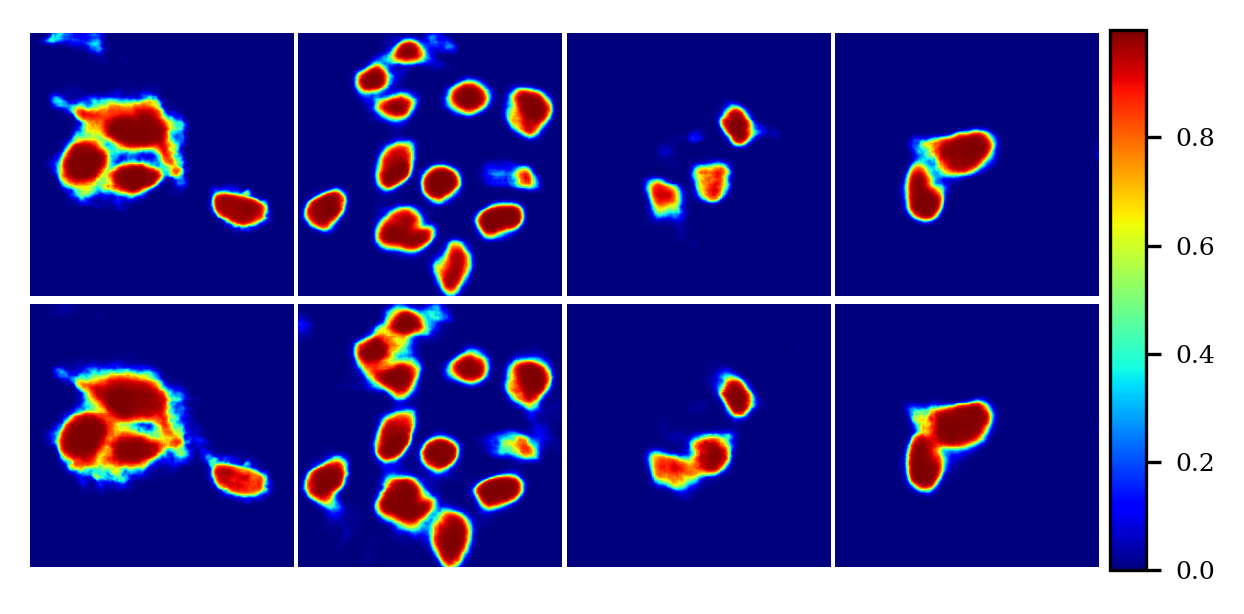
\includegraphics[width=\textwidth]{figures/130_methods/weigths_effect.png}
\caption{\textbf{Weight map effect}. 
Predicted heatmaps obtained with c-ResUnet (top row) and c-ResUnet (no WM).} 
\label{fig:weigths_effect}
% \end{wrapfigure}
\end{figure}
\begin{figure}
\centerline{
     \begin{subfigure}[]{0.55\textwidth}
         \centering
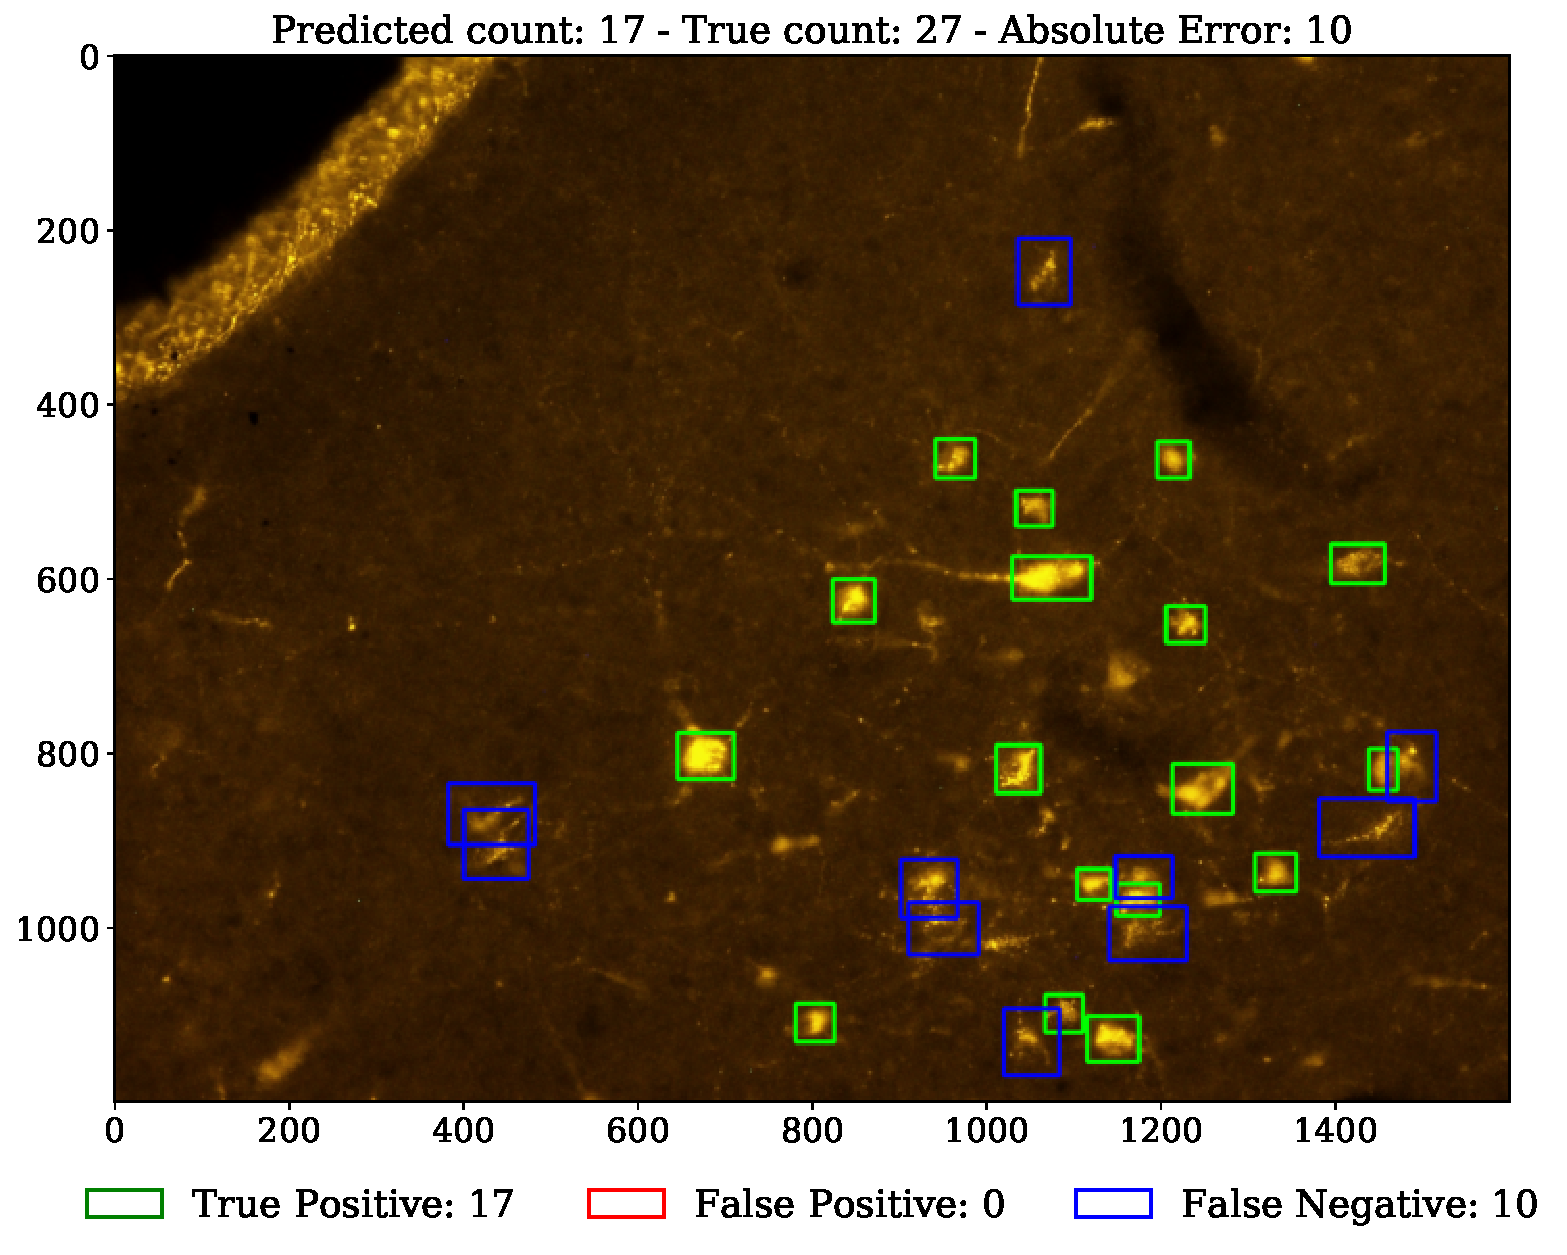
\includegraphics[width=\textwidth]{figures/140_results/pred_ResUnet_noAO:281.eps}
        \caption{
        % c-ResUnet (no AO) prediction on artifact
        }
        \label{fig:predictions:noAO}
     \end{subfigure}
          \begin{subfigure}[]{0.55\textwidth}
         \centering
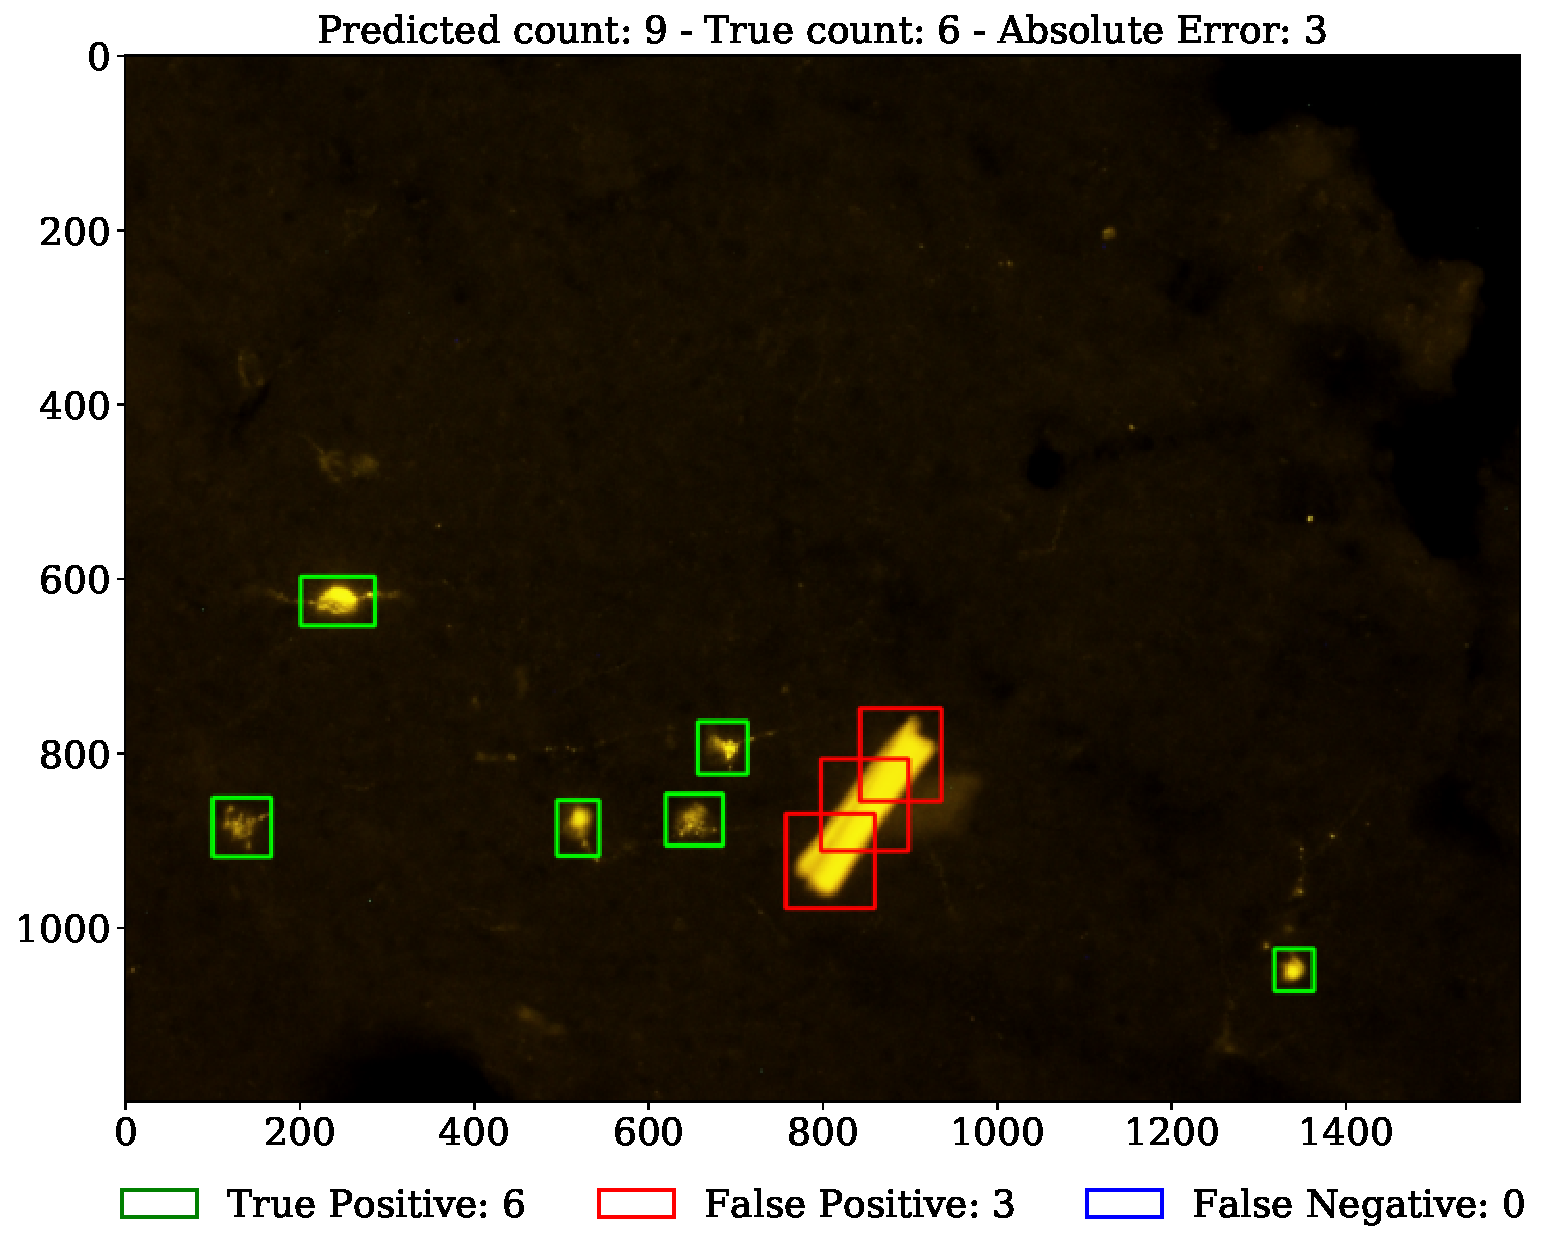
\includegraphics[width=\textwidth]{figures/140_results/pred_ResUnet:254.eps}
        \caption{
        % c-ResUnet prediction on artifact
        }
        \label{fig:predictions:artifact}
     \end{subfigure}
}
\centerline{
          \begin{subfigure}[]{0.55\textwidth}
         \centering
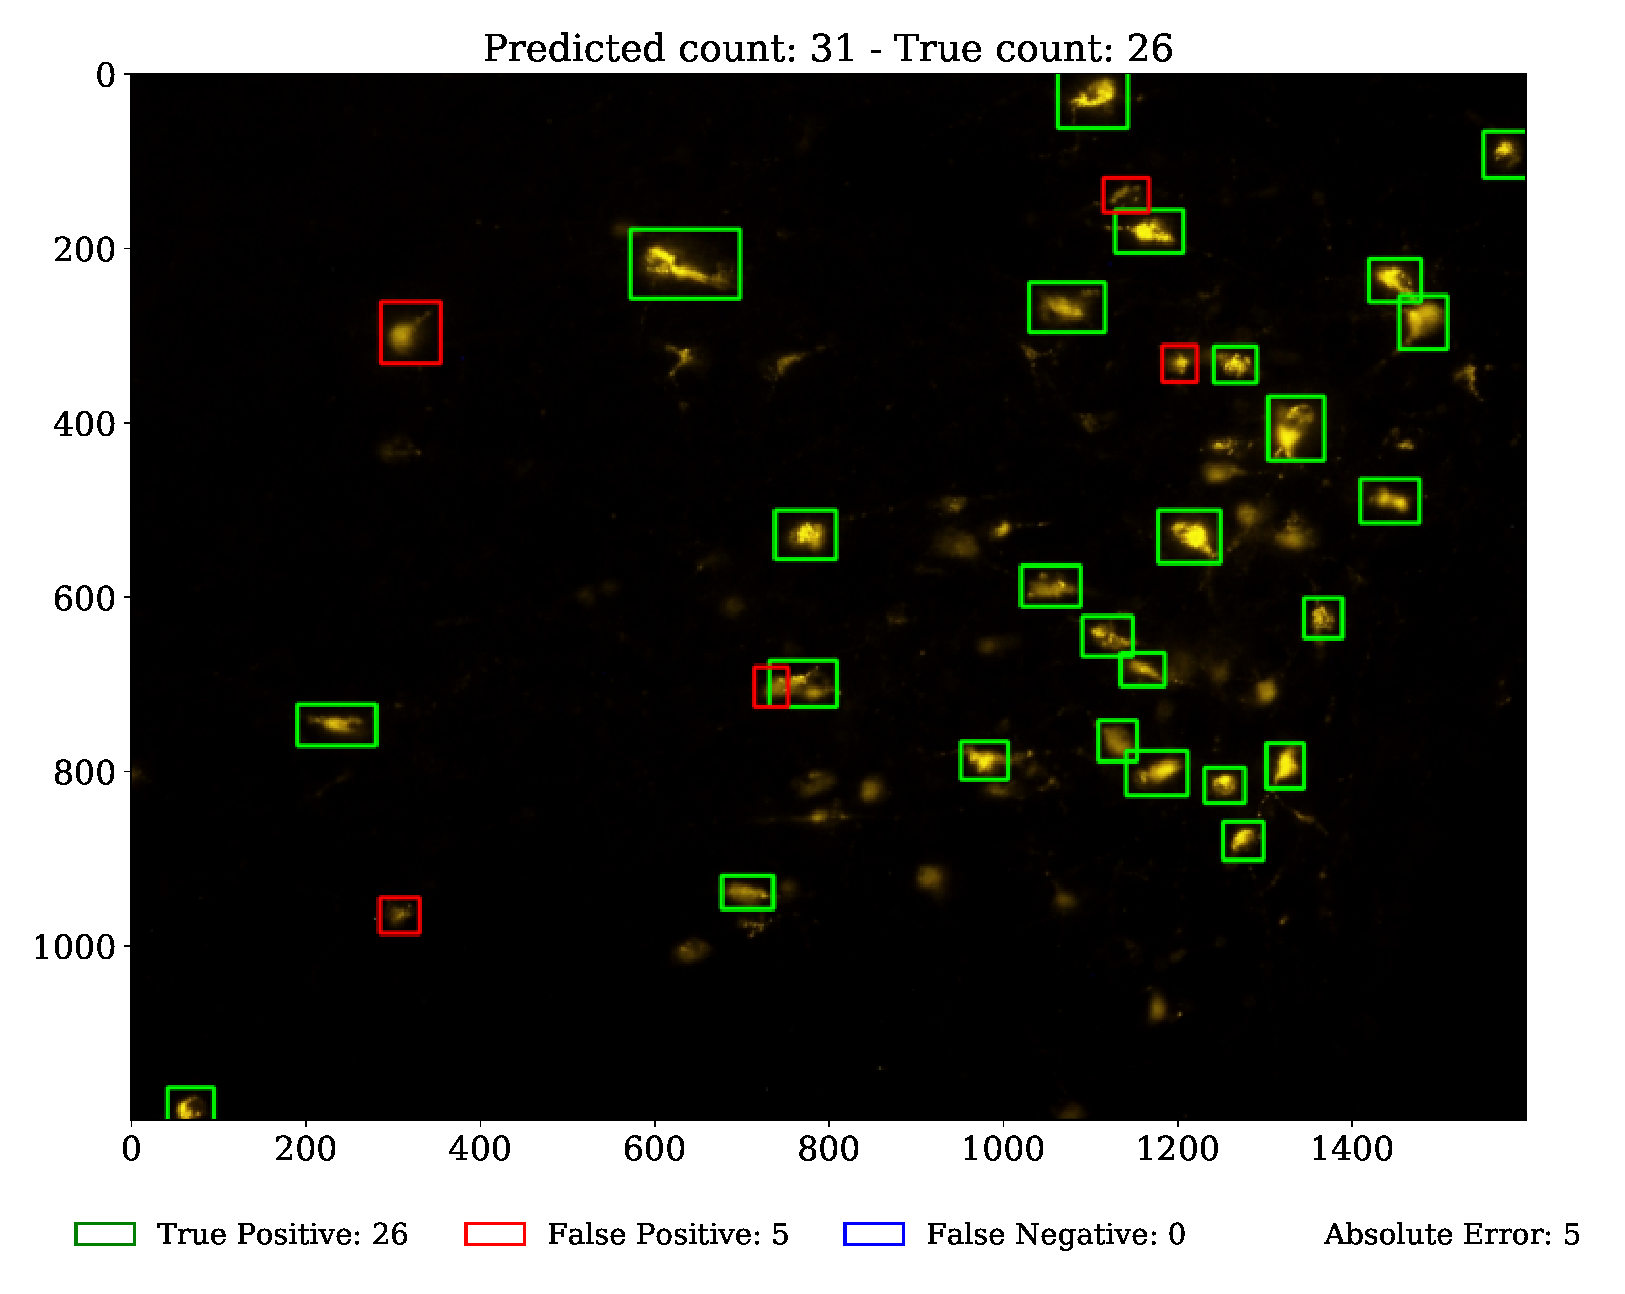
\includegraphics[width=\textwidth]{figures/140_results/pred_ResUnet:168.eps}
        \caption{
        % c-ResUnet prediction on artifact
        }
        \label{fig:predictions:false-positives}
     \end{subfigure}
       \begin{subfigure}[]{0.55\textwidth}
         \centering
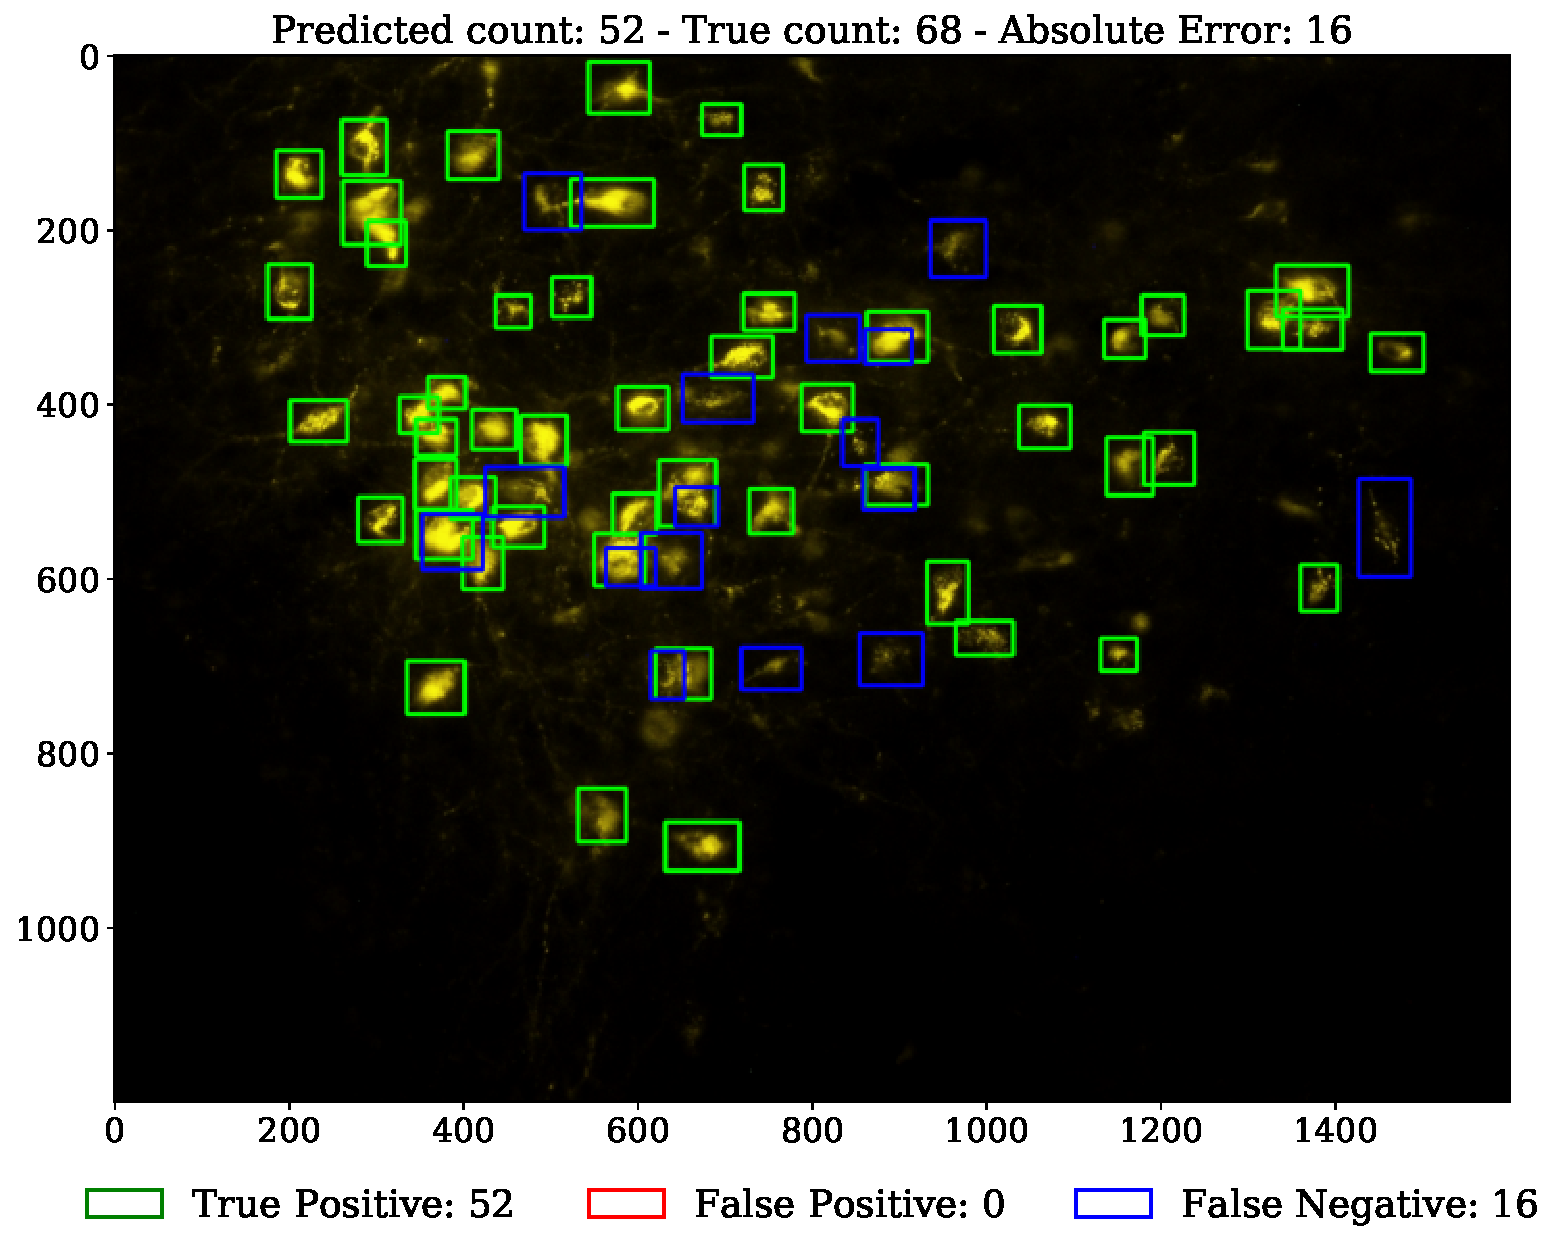
\includegraphics[width=\textwidth]{figures/140_results/pred_ResUnet:278.eps}
        \caption{
        % c-ResUnet prediction on artifact
        }
        \label{fig:predictions:false-negatives}
     \end{subfigure}
}
\caption{\textbf{Results on test images}. 
% Top row illustrates AO effect. 
The c-ResUnet (no AO) correctly handles evident artifacts (\ref{fig:predictions:noAO}, top left corner), while the c-ResUnet fails with more problematic structures (\ref{fig:predictions:artifact}).
% Bottom row highlights c-ResUnet predictive ability. 
Notice how false positives (\ref{fig:predictions:false-positives}, red boxes) look like target cells. Likewise, the objects discarded (\ref{fig:predictions:false-negatives}, blue boxes) are similar to other stains that were not annotated.
} 
\label{fig:predictions}
\end{figure}